\graphicspath{{solutiondevelopment/fig/}}

\chapter{Solution development}
\label{chap:solutiondevelopment}
The goal of this project is to develop a tool for calculating the low frequency mean square flux noise figure given a SQUID's geometry with the use of the software package InductEx. In \cite{fluxNoiseSquidsStevenAnton} the authors propose a framework for implementing such a tool but then only applied the method to a square washer. As pointed out in \cite{fluxNoiseSquidsStevenAnton} the other numerical technique suffers from performance and resolution problems. This section will serve to communicate the design effort by systematically breaking down the problem and motivating design decisions along the way. I will start by first identifying the design requirements.

\section{Design goals}
In section \ref{chap:litreview} it was made clear that the origin of the low frequency noise is still unknown. The S.M. Anton et al. pointed concluded \cite{fluxNoiseSquidsStevenAnton} by remarking on the flexibility of his numerical framework. It can readily be adapted, with only minor modifications to the framework, to account for a variety of different models. As such a major design requirement is to reflect the flexibility of the framework within the design of the tool.
The second and perhaps most obvious design goal is that the tool must be fast. The end user of such a tool is a SQUID designer. As discussed in chapter \ref{chap:litreview} the design of SQUID systems relies heavily on computational methods. The non-linear nature of the Josephson junctions makes analytical solutions to design problems not feasible. In such cases the designer often has to rely on an iterative approach to design.
The tool must be generalized to work on any geometry one might give it.
The last design goal is to use TetraHenry for the calculation of the magnetic flux density. 

\section{High Level System Design}
The project calls for the development of 3 independent modules. The first module must be able to take a certain geometry and extract the mesh of the surface of said geometry as this will be used for calculation of the surface magnetic flux density. The second module must implement mesh refinement around regions of rapidly varying currents across mesh nodes. The last module must implement the numerical framework as described by \cite{fluxNoiseSquidsStevenAnton} using the simulation results from InductEx. \par
To understand the role the tool will play one must first understand the basic interactions a user might have with the software package. One must also understand what each entity requires as input and what its outputs are. Figure \ref{fig:Inductexproc} summaries this and figure \ref{fig:ProcessFlow} shows how each module interacts with this process.
\begin{figure}[h]
    \centering
    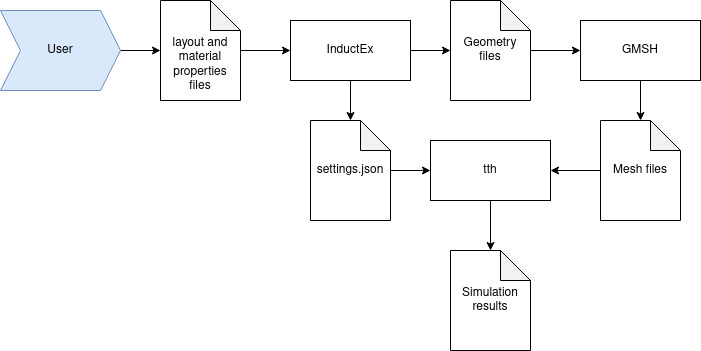
\includegraphics[width=0.8\linewidth]{Inductexproc}
    \caption{A process showing how the average user might interact with InductEx and TetraHenry. The figure also shows typical input and output files at each entity in the process.}
    \label{fig:Inductexproc}
\end{figure}
\begin{figure}[h]
    \centering
    \includegraphics[width=0.8\linewidth]{ProcessFlow}
    \caption{A process chart showing how the user interacts with InductEx as well as how each module will interact with this process.}
    \label{fig:ProcessFlow}
\end{figure}

\subsection{InductEx}
InductEx has gone through major changes since the publication of \cite{fluxNoiseSquidsStevenAnton}. InductEx is a powerful tool that supports a large feature set. Most of these features are not relevant to this project. I only require magnetic field calculations for the surface of the conductor, so these features will mostly be ignored.

\subsection{GMSH}
GMSH is an open-source tool that is used to discretize geometry \cite{GMSH}. GMSH supports a scripting language to specify geometry before discretization. InductEx generates a file in this scripting language to be run through GMSH to generate a finite element mesh for use in TetraHenry. GMSH typically accepts a ".geo" file and outputs a ".msh" file. In GMSH you specify the geometry in a hierarchical fashion. You start by defining the lowest dimension elements and build up the geometry from there. In GMSH the lowest dimension entity is the point and is referred to as a "0 dimensional" entity. Higher dimensional entities are bounded by lower dimensional entities for example: A volume is bounded by a set of 2 dimensional surfaces. A surface is defined by a closed loop of 1 dimensional curves. A curve is defined by the 0 dimensional points. This fact will become useful in the design of the GMSH extraction module. GMSH entities are added to physical groups specified by the user. Physical groups are essentially just names for collections of mesh entities. The most common use of physical groups is to use them to define material properties. The implementation and use of physical groups depend on the context GMSH is used in. In TetraHenry physical groups are used to specify a number of things but most relevant to this project, it is used to specify the mesh entities to be used for field calculations. 

\subsection{TetraHenry (TTH)}
TetraHenry is the numerical field solver that will be used to calculate the surface magnetic flux density. This project will interact directly with TetraHenry. Refer to appendix \textcolor{red}{Insert sample json file in appendix} for the template ".json" input file used. Depending on the setup of the simulation, TetraHenry will write the results to a folder titled output. When specified, TetraHenry will write the magnetic flux density to a "vtk" file as an unstructured grid. 

\section{Detailed Design}
\subsection{Choice of programming language}
The visualisation tool kit (VTK) is an open-source modelling and visualisation tool kit. As TetraHenry reports simulation results in the VTK file format it is necessary that the language of choice supports the VTK library. Of the rich variety of programming and scripting languages available, few match the design requirements. The VTK library is only supported by python and C++. Python is a high level interpreted language and is often used for scientific computing. Python is very flexible but suffers from performance issues due to it being interpreted. C++ is a lower level compiled programming language that is generally regarded as a "fast" programming language. This is largely due to the fact that it does not have the overhead that comes with an interpreted language. In order to meet performance goals C++ will be used.

\subsection{The noise extraction module}
This module is based on the work done by \cite{fluxNoiseSquidsStevenAnton}. This module will be implemented as a command line tool. The module receives the path to a VTK file which defines an unstructured grid and the total current circulating in the SQUID washer as command line arguments. The unstructured grid specifies the individual mesh elements (triangles)  that the surface of the SQUID washer in question consists of. Additionally, each node of each mesh element has a vector associated with it representing the magnetic flux density at the location of said node. \par
This module effectively implements equation \ref{eq:MSFNfromBfield} numerically. Expanding equation \ref{eq:MSFNfromBfield}:


\begin{equation}
    \langle \Phi ^2 \rangle = \frac{N\mu_B^2}{3I^2} \frac{\iint \Vec{B(\Vec{r})}\cdot\Vec{B(\Vec{r})} ds}{\iint ds}
    \label{eq:MSFNexpanded}
\end{equation}

Noting that in equation \ref{eq:MSFNexpanded} $N/\iint ds = \sigma$ and therefore the bottom integral can be eliminated \cite{fluxNoiseSquidsStevenAnton}. Next we discretize the integral: 
\begin{equation}
    \langle \Phi ^2 \rangle = \frac{\sigma\mu_B^2}{3I^2}\sum_{n}^{N_{\text{nodes}}}[\Vec{B}(\Vec{r_n})\cdot\Vec{B}(\Vec{r_n})]A_n
    \label{eq:MSFNdiscrete}
\end{equation}
In equation \ref{eq:MSFNdiscrete} $A_n$ refers to the area associated with the $n_{th}$ node. The method for determining $A_n$ is discussed at a later stage in the design. Similarly, $\Vec{r_n}$ refers to the vector position of the $n_{th}$ node in the unstructured grid. The basic algorithm then follows as such:
\begin{algorithm}
\begin{algorithmic}
    \State $N \gets \text{Number of points in grid}$
    \State $pts \gets \text{list of all points}$
    \State $A \gets $ list of all areas
    \State $i \gets 0$ 
    \While{$i < N$}
        \State $A_n \gets A[i]$
        \State $r_n \gets pts[i]$ 
        \State $\Phi^2 \gets \Phi^2 + \Vec{B}(\Vec{r_n})\cdot \Vec{B}(\Vec{r_n}) A_n$ 
    \EndWhile
    \State $\Phi^2 \gets \Phi^2 \cdot \frac{\sigma\mu_B^2}{3I^2}$ 
\end{algorithmic}
\caption{The algorithm for evaluating the discretized integral}
\end{algorithm}


